\documentclass[12pt]{beamer}
\usetheme{CambridgeUS}
\usepackage[utf8]{inputenc}
\usepackage{amsmath}
\usepackage{amsfonts}
\usepackage{amssymb}
\author{Kleiner et al.}
\title{A scalable bootstrap for massive data}
%\setbeamercovered{transparent} 
%\setbeamertemplate{navigation symbols}{} 
%\logo{} 
%\institute{} 
%\date{} 
%\subject{} 
\begin{document}

\begin{frame}
\titlepage
\end{frame}

%\begin{frame}
%\tableofcontents
%\end{frame}

\section{Introduction}

\begin{frame}{Introduction}
Two recent trends are worthy of attention in this regard.

{\bf First,} the growth in size of data sets is
accelerating, with ‘massive’ data sets becoming increasingly prevalent.

{\bf Second,} computational resources are shifting towards parallel and distributed architectures, with multicore and cloud
computing platforms providing access to hundreds or thousands of processors.

{\bf However}, from an
inferential point of view, it is not yet clear how statistical methodology will transport to a world
involving massive data on parallel and distributed computing platforms.

\end{frame}



\begin{frame}{Introduction}
The bootstrap would seem ideally suited to exploiting the trend towards
parallel and distributed computing: one might imagine using different processors or compute
nodes to process different bootstrap resamples independently in parallel.

However, in the massive data setting,
computation of even a single point estimate on the full data set can be quite computationally
demanding.
\end{frame}

\begin{frame}{Introduction}
Another landmark in the development of simulation-based inference is subsampling and the closely related m out of n bootstrap.
\begin{itemize}
\item finite sample behaviour can be worse, and their
success is sensitive to the choice of resample (or subsample) size.
\item Although schemes have been
proposed for data-driven selection of an optimal resample size (Bickel and Sakov, 2008), they
require significantly greater computation which may eliminate any computational gains.
\end{itemize}
\end{frame}

\begin{frame}{Introduction}

{\bf bag of little bootstrap : BIB}

Subsample + Boostrap+ Divide and Conquer
\end{frame}


\section{Bag of little bootstrap}
\begin{frame}{Setting and notation}
\begin{itemize}
\item We assume that we observe a sample $X_1,\dots,X_n$ drawn i.i.d. from some unknown distribution $P$
\item We denote $\mathbb{P}_{n}=n^{-1} \sum_{i=1}^{n} \delta_{X_{i}}$, the corresponding empirical distribution.
\item On the basis of the observed data, we form an estimate $\hat{\theta}_{n}=\hat{\theta}_{n}\left(\mathbb{P}_{n}\right)$ of some unknown population value $P(\theta)$.
\item Our end goal is to obtain an assessment $\xi\{Q_n(P)\}$ of the quality of the estimate $\hat{\theta}_{n}\left(\mathbb{P}_{n}\right)$, which consists of a summary of the distribution $Q_n(P)$ of
some quantity $u(\mathbb{P}_n, P)$ \item The choice of $u$ depends on one’s inferential goals.
\end{itemize}

\end{frame}


\begin{frame}{Setting and notation}
In practice, we cannot compute $\xi\{Q_n(P)\}$ directly because $P$ and $Q_n(P)$ are unknown, and so we must estimate $\xi\left\{Q_{n}(P)\right\}$ on the basis of a single observed
data set.

Under this notation, the bootstrap simply computes the plug-in approximation $\xi\left\{Q_{n}\left(\mathbb{P}_{n}\right)\right\} \approx \xi\{Q_n(P)\}$

Note that the
vast majority of the bootstrap’s computational cost lies in the repeated computation of values
of $u$, which in turn requires costly repeated computation of estimates $\hat{\theta}_n(\mathbb{P}_n^{*})$ on resamples.
\end{frame}


\begin{frame}{BLB}
\begin{itemize}
\item Given a subset size $b<n$, the BLB samples $s$ subsets of size $b$ without replacement from the original $n$ data points, uniformly at random (one can also impose the constraint
that the subsets are disjoint).
\item Let $\mathcal{I}_{1}, \ldots, \mathcal{I}_{s} \subset\{1, \ldots, n\}$ be the corresponding index sets.
\item Let $\mathbb{P}_{n, b}^{(j)}=b^{-1} \Sigma_{i \in \mathcal{I}_{j}} \delta_{X_{i}}$ denote the empirical distribution corresponding
to subset j.
\item The BLB’s estimate of $\xi\{Q_n(P)\}$ is then given by
\begin{equation}\tag{1}
s^{-1} \sum_{j=1}^{s} \xi\left\{Q_{n}\left(\mathbb{P}_{n, b}^{(j)}\right)\right\}.
\end{equation}
\end{itemize}
\end{frame}

\begin{frame}{BLB}
Although the terms $\xi\left\{Q_{n}\left(\mathbb{P}_{n, b}^{(j)}\right)\right\}$ in expression (1) cannot be computed analytically in general, they can be computed numerically via straightforward Monte Carlo approximation in the manner
of the bootstrap.

For each term $j$, repeatedly resample n points IID from $\mathbb{P}_{n, b}^{(j)}$ form the
empirical distribution $\mathbb{P}^{*}_{n,b}$ and compute $u\left(\mathbb{P}_{n, b}^{*}, \mathbb{P}_{n, b}^{(j)}\right)$ for each resample, form the empirical
distribution $\mathbb{Q}_{n,j}^{*}$ of the computed u-values, and compute $\xi\left(\mathbb{Q}_{n, j}^{*}\right) \approx \xi\left\{Q_{n}\left(\mathbb{P}_{n, b}^{(j)}\right)\right\}$.
\end{frame}

\begin{frame}{Algorithm 1: the BLB}
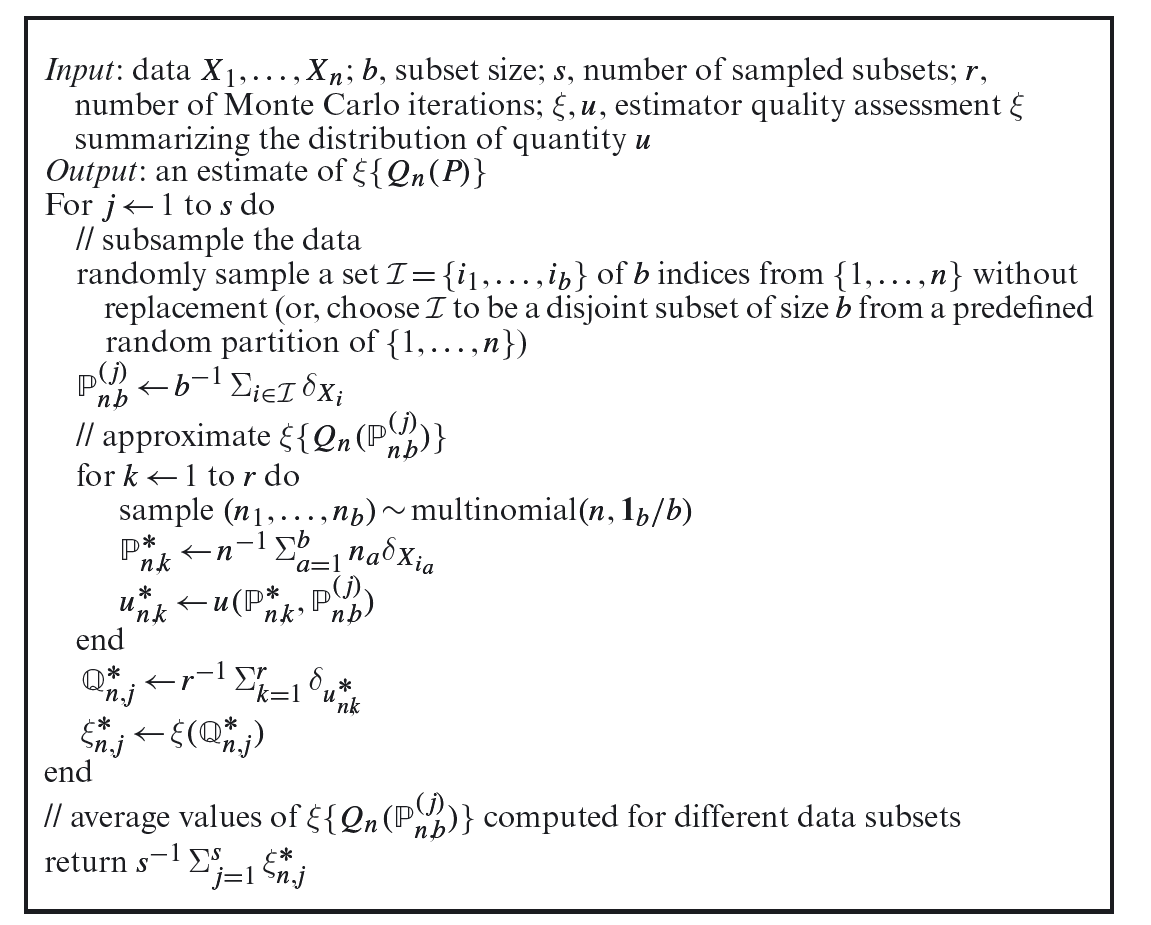
\includegraphics[scale=0.9]{table1.png}
\end{frame}

\begin{frame}{The BLB}
The BLB straightforwardly permits computation on multiple (or even all) subsamples
and resamples simultaneously in parallel: because BLB subsamples and resamples can
be significantly smaller than the original data set, they can be transferred to, stored by and
processed on individual (or very small sets of) compute nodes.
\end{frame}

\section{Consistency and higher order correctness}
\begin{frame}{Theorem 1}
Suppose that $\hat{\theta}_{n}\left(\mathbb{P}_{n}\right)=\phi\left(\mathbb{P}_{n}\right)$ and $\theta(P)=\phi(P)$, where $\phi$ where $\phi$ is Hadamard differentiable
at P tangentially to some subspace, with $P,\mathbb{P}_n$ and $\mathbb{P}_{n,b}^{(j)}$ viewed as maps from some Donsker
class $\mathcal{F}$ to $\mathbb{R}$ such that $\mathcal{F}_{\delta}$ is measurable for every $\delta>0$, where $\mathcal{F}_{\delta}=\left\{f-g: f, g \in \mathcal{F}, \rho_{P}(f-g)<\delta\right\}$. Additionally, assume that $\xi\left\{Q_{n}(P)\right\}$ is a function of
the distribution of $u\left(\mathbb{P}_{n}, P\right)=n^{1 / 2}\left\{\phi\left(\mathbb{P}_{n}\right)-\phi(P)\right\}$ which is continuous in the space of such
distributions with respect to a metric that metrizes weak convergence. Then,
$$
s^{-1} \sum_{j=1}^{s} \xi\left\{Q_{n}\left(\mathbb{P}_{n, b}^{(j)}\right)\right\}-\xi\left\{Q_{n}(P)\right\} \stackrel{\mathrm{P}}{\rightarrow} 0
$$
as $n \to \infty$, for any sequence $b \to \infty$  and any fixed $s$.
\end{frame}

\begin{frame}{Theorem 2}
Suppose that $\xi\left\{Q_{n}(P)\right\}$ admits an expansion as an asymptotic series
$$
\xi\left\{Q_{n}(P)\right\}=z+\frac{p_{1}}{\sqrt{n}}+\cdots+\frac{p_{k}}{n^{k / 2}}+o\left(\frac{1}{n^{k / 2}}\right),
$$
where $z$ is a constant independent of $P$ and the $p_k$ are polynomials in the moments of P. Additionally, assume that the empirical version of $\xi\{Q_n(P)\}$ for any $j$ admits a similar expansion
$$
\xi\left\{Q_{n}\left(\mathbb{P}_{n, b}^{(j)}\right)\right\}=z+\frac{\hat{p}_{1}^{(j)}}{\sqrt{n}}+\ldots+\frac{\hat{p}_{k}^{(j)}}{n^{k / 2}}+o_{P}\left(\frac{1}{n^{k / 2}}\right).
$$

\end{frame}
\begin{frame}{Therem 2 Continue}
Then, assuming that $b \le n$ and $E\left(\hat{p}_{k}^{(1)}\right)^{2}<\infty$ for $k \in \{1,2\}$,
$$
\begin{aligned}
&\left|s^{-1} \sum_{j=1}^{s} \xi\left\{Q_{n}\left(\mathbb{P}_{n, b}^{(j)}\right)\right\}-\xi\left\{Q_{n}(P)\right\}\right|\\
&=\sum_{k=1}^{2} O_{P}\left[\frac{\sqrt{\left\{\operatorname{var}\left(\hat{p}_{k}^{(1)}-p_{k} | \mathbb{P}_{n}\right)\right\}}}{n^{k / 2} \sqrt{s}}\right]+O_{P}\left(\frac{1}{n}\right)+O\left(\frac{1}{b \sqrt{n}}\right)
\end{aligned}
$$
\end{frame}
\begin{frame}{Theorem 2 Continue}
Therefore, taking $s=\Omega\left[\max \left\{n \operatorname{var}\left(\hat{p}_{1}^{(I)}-p_{1} | \mathbb{P}_{n}\right), \operatorname{var}\left(\hat{p}_{2}^{(1)}-p_{2} | \mathbb{P}_{n}\right)\right\}\right]$ and $b=\Omega(\sqrt{n})$ yields
$$
\left|s^{-1} \sum_{j=1}^{s} \xi\left\{Q_{n}\left(\mathbb{P}_{n, b}^{(j)}\right)\right\}-\xi\left\{Q_{n}(P)\right\}\right|=O_{P}\left(\frac{1}{n}\right),
$$
in which case the BLB enjoys the same level of higher order correctness as the bootstrap.
\end{frame}

\begin{frame}{Theorem 3}
Theorem 3. Under the assumptions of theorem 2, and assuming that the BLB uses disjoint
random subsets of the observed data (rather than simple random subsamples), we have

$$
\left|s^{-1} \sum_{j=1}^{s} \xi\left\{Q_{n}\left(\mathbb{P}_{n, b}^{(j)}\right)\right\}-\xi\left\{Q_{n}(P)\right\}\right|=O_{P}\left\{\frac{1}{\sqrt{(n b s)}}\right\}+O\left(\frac{1}{b \sqrt{n}}\right),
$$
Therefore, if $s\sim n/b$ and $b=\Omega(\sqrt{n})$, then
$$
\left|s^{-1} \sum_{j=1}^{s} \xi\left\{Q_{n}\left(\mathbb{P}_{n, b}^{(j)}\right)\right\}-\xi\left\{Q_{n}(P)\right\}\right|=O_{P}\left(\frac{1}{n}\right).
$$
\end{frame}

\section{Simulation Study}
\begin{frame}{Simulation}
\begin{itemize}
\item We consider two different settings: regression and classification.
\item For both setting, the data have the form $X_{i}=\left(\tilde{X}_{i}, Y_{i}\right) \sim P$, IID for $i=1,\dots,n$ where $\tilde{X}_{i}\in \mathbb{R}^d$; $Y_i \in \mathbb{R}$ for regression whereas $Y_i \in\{0,1\}$ for classification.
\item In each case, $\hat{\theta}_n$ estimates a parameter vector in $\mathbb{R}^d$ for a linear or
generalized linear model of the mapping between $\tilde{X}_{i}$ and $Y_i$.
\end{itemize}
\end{frame}

\begin{frame}{Simulation}
\begin{itemize}
\item We define $\xi$ as a procedure that computes a set of marginal 95\% confidence interval, one for each element of the estimated
parameter vector.
\item In particular, given the distribution $Q_n(P)$ of $u\left(\mathbb{P}_{n}, P\right)=\hat{\theta}_{n}\left(\mathbb{P}_{n}\right)$, $\xi$ forms the boundaries of the relevant confidence intervals as the 2.5th
and 97.5th percentiles of the marginal componentwise distributions defined by $Q_n(P)$.
\item Averaging
across these confidence intervals in the averaging step of the BLB simply consists in averaging
these percentile estimates.
\end{itemize}
\end{frame}

\begin{frame}{Simulation}
\begin{itemize}
\item To evaluate the various quality assessment procedures on a given estimation task and true
underlying data distribution P, we first compute the ground truth $\xi\{Q_n(P)\}$ by generating 2000
realizations of data sets of size n from P, computing $\hat{\theta}_n$ on each, using this collection of $\hat{\theta}_n$s to form a high fidelity approximation to $Q_n(P)$.
\item Each estimate is evaluated on the basis of the average relative deviation of its componentwise confidence intervals' widths from the corresponding true width: $|c-c_0|/c_0$.
\item For the BLB, the b out of n bootstrap, and subsampling, we consider $b=n^{\gamma}$ with $\gamma\in \{0.5,0.6,0.7,0.8,0.9 \}$; we use $r=100$ in all runs of BLB. 
\end{itemize}
\end{frame}


\begin{frame}{Simulation: Regression}
\begin{itemize}
\item In the regression setting, we generate each data set from a true underlying distribution $P$ consisting of either a linear model $Y_i=\tilde{X}_i1_{d}+\varepsilon_i$ or a model $Y_{i}=\tilde{X}_{i}^{\mathrm{T}} \mathbf{1}_{d}+\tilde{X}_{i}^{\mathrm{T}} \tilde{X}_{i}+\varepsilon_{i}$ having
a quadratic term, with $d=1000$ and $n=20000$.
\item The $\tilde{X}_i$ and $\varepsilon_i$ are drawn independently from one of the following pairs of distributions: 
\begin{itemize}
\item $\tilde{X}_i\sim normal(0,1_{d})$ with $\varepsilon_i \sim normal(0,10)$,
\item $\tilde{X}_{i,j}\sim StudentT(3)$ IID with $\varepsilon_i \sim normal(0,10)$,
\item $\tilde{X}_{i,j}\sim gamma\{1+5(j-1)/\max(d-1,1),2\}-2\{1+5(j-1)/\max(d-1,1),2\}$ IID with $\varepsilon_i \sim gamma(1,2)-2$.
\end{itemize} 
\end{itemize}
\end{frame}

\begin{frame}{Simulation : Regression}
\href{fig1.png}{\color{blue} Fig 1: Relative error versus processing time for the regression setting}
\end{frame}

\begin{frame}{Simulation: Classification}
\begin{itemize}
\item We generate each data set considered from either a linear model $Y_i\sim Bernuoulli[\{1+\exp(-\tilde{X}_i^T1_{d})\}^{-1}]$ or a model $Y_i\sim Bernuoulli[\{1+\exp(-\tilde{X}_i^T1_{d}-\tilde{X}_i^T\tilde{X}_i)\}^{-1}]$ having a quadratic term, with $d=10$.
\item We use the same distribution on $\tilde{X}_i$ that were used in the regression setting.
\item Our estimator,under both the linear and the quadratic data-generating distributions, consists of a linear logistic regression fit via Newton's method. 
\end{itemize}
\end{frame}

\begin{frame}{Simulation: Classification}
\href{fig2.png}{\color{blue} Fig 2: Relative error versus processing time for the classification setting}

\href{fig3.png}{\color{blue} Fig 3: Relative error versus processing time for the classification setting}
\end{frame}

\begin{frame}{Computation Scalability}
\begin{itemize}
\item Now, we use $d=3000$ and $n=6$ million so the size of full observed data set ia approximately 150 Gbytes.
\item $r=50,s=5$ and $b=n^{0.7}$.
\item 10 worker nodes, each having 6 Gbtyes of memory and eight compute cores.
\item \href{fig4.png}{\color{blue} Fig 4: Relative error versus time on 150 Gbytes of data}
\end{itemize}
\end{frame}

\begin{frame}{Tuning Parameter}
The BLB requires the specification of tuning parameters controlling the number of subsamples and resamples processed.

\href{fig5.png}{\color{blue} Fig 5: Results for BIB tuning parameter selection}
\end{frame}

\begin{frame}{Real Data}
\begin{itemize}
\item University of California at Irvine connnect4 data set.
\item The model is logistic regression with $d=42 , n=67557$.
\item We now report the average absolute confidence interval width.
\item \href{fig6.png}{\color{blue} Fig 6: Average (across dimensions) absolute confidence interval width versus processing time}
\end{itemize}
\end{frame}

\begin{frame}{Time Series}
\begin{itemize}
\item Variants of the bootstrap such as the moving block bootstrap and the stationary bootstrap  have been proposed to handle other data analysis settings such as that of time series.
\item These bootstrap variants can be used within the BLB.
\end{itemize}
\end{frame}

\begin{frame}{Time Series}
\begin{itemize}
\item To extend the BLB in this manner, we must simply alter both the subsample selection mechanism and the resample generation mechanism such that both of these processes respect the underlying data-generating process.
\item In particular,for stationary time series data it suffices to select each subsample as a(uniformly)randomly positioned block of length b within the observed time series of length n. 
\item Given a subsample of size b, we generate each resample by applying the stationary bootstrap to the subsample to obtain a series of length n. 
\end{itemize}
\end{frame}
 
 
\begin{frame}{Time Series}
 Given a $p\in [0,1]$, we first select uniformly at random a data point in the subsample series and then repeat the following process until we have amassed a new series of length $n$:   with probability 1-p we append to our resample the next point in the subsample  series(wrapping around to the beginning if we reach the end of the subsample series),and with probability p we (uniformly at random) select and append a new point in the subsample series. 
\end{frame}

\begin{frame}{Time Series}
\begin{itemize}
\item We generate observed data consisting of a stationary time series 
$X_1,\dots,X_n\in \mathbb{R}$ where $X_t=Z_t+Z_{t-1}+Z_{t-2}+Z_{t-3}+Z_{t-4}$ and $Z_t$ are drawn independently from a normal(0,1)distribution.
\item We consider the task of estimating the standard deviation of the rescaled mean $\sum_{t=1}^n X_t/\sqrt{n}$.
\item We set $p=0.1, n=5000$.
\end{itemize}
\end{frame}
\begin{frame}{Time Series}
\begin{center}
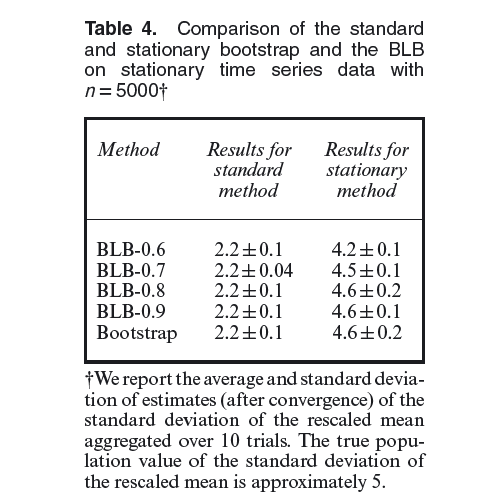
\includegraphics[scale=1]{table4.png} 
\end{center}
\end{frame}
\end{document}